

\documentclass[12pt]{extarticle}
%Some packages I commonly use.
\usepackage[english]{babel}
\usepackage{graphicx}
\usepackage{framed}
\usepackage[normalem]{ulem}
\usepackage{amsmath}
\usepackage{amsthm}
\usepackage{amssymb}
\usepackage{amsfonts}
\usepackage{enumerate}
\usepackage[utf8]{inputenc}
\usepackage[top=1 in,bottom=1in, left=1 in, right=1 in]{geometry}
\usepackage{tikz}
\usepackage{lineno}
\usepackage{hyperref}
\usepackage[english]{babel}
\usepackage{seqsplit}
\usepackage[nottoc]{tocbibind} 
\usepackage[utf8]{inputenc}

\newcommand{\cvec}[1]{{\mathbf #1}}
\newcommand{\murgg}{\Gamma(K^{ur}/K)}
\newcommand{\rvec}[1]{\vec{\mathbf #1}}
\newcommand{\ihat}{\hat{\textbf{\i}}}
\newcommand{\jhat}{\hat{\textbf{\j}}}
\newcommand{\khat}{\hat{\textbf{k}}}
\newcommand{\minor}{{\rm minor}}
\newcommand{\trace}{{\rm trace}}
\newcommand{\spn}{{\rm Span}}
\newcommand{\rem}{{\rm rem}}
\newcommand{\ran}{{\rm range}}
\newcommand{\range}{{\rm range}}
\newcommand{\mdiv}{{\rm div}}
\newcommand{\proj}{{\rm proj}}
\newcommand{\R}{\mathbb{R}}
\newcommand{\N}{\mathbb{N}}
\newcommand{\F}{\mathbb{F}}
\newcommand{\Q}{\mathbb{Q}}
\newcommand{\Z}{\mathbb{Z}}
\newcommand{\co}{\mathcal{O}}
\newcommand{\GG}{\Gamma(K/\mathbb{Q})}
\newcommand{\spl}{split(f(x),\mathbb{Q})}
\newcommand{\<}{\langle}
\renewcommand{\>}{\rangle}
\renewcommand{\emptyset}{\varnothing}
\newcommand{\attn}[1]{\textbf{#1}}
\theoremstyle{definition}
\newtheorem{theorem}{Theorem}
\newtheorem{corollary}{Corollary}
\newtheorem*{definition}{Definition}
\newtheorem{proposition}{Proposition}
\newtheorem*{example}{Example}
\newtheorem{lemma}{Lemma}
\newtheorem*{note}{Note}
\newtheorem{exercise}{Exercise}
\newcommand{\bproof}{\bigskip {\bf Proof. }}
\newcommand{\eproof}{\hfill\qedsymbol}
\newcommand{\Disp}{\displaystyle}
\newcommand{\qe}{\hfill\(\bigtriangledown\)}
\newcommand{\lb}{\left(}
\newcommand{\rb}{\right)}
\newenvironment{polynomial}
  {\par\vspace{\abovedisplayskip}%
   \setlength{\leftskip}{\parindent}%
   \setlength{\rightskip}{\leftskip}%
   \medmuskip=4mu plus 2mu minus 2mu
   \binoppenalty=0
   \noindent$\displaystyle}
  {$\par\vspace{\belowdisplayskip}}
\setlength{\columnseprule}{1 pt}

\title{Extensions of number fields with small ramification}

\author{Samuel Bodansky}
\date{March 2019}

\begin{document}
%!TEX root = ../main.tex
\maketitle

\section{Notation}
\begin{enumerate}
    \item K is a number field, h(K) is its class number and Cl(K) is its ideal class group.
    \item $d_K$ is the discriminant of K.
    \item $K^{ur}$ is the maximally unramified extension of K.
    \item $K^{tur}$ is the maximal tamely unramified extension of K.
    \item $n_K$ is the degree of the extension $K:\mathbb{Q}$.
    \item $\bar{K}$ denotes the Galois closure of K.
    \item KL denotes the compositum of two number fields K and L.
    \item $rd_K$ is the root discriminant of K, $|d_K|^\frac{1}{n_K}$ .
    \item $G_K$ is the Galois group $\Gamma(\bar{K}:K)$
    \item $G_K^{ur}$ is the Galois group $\Gamma(K^{ur}:K)$
    \item $C_K$ is the class field group of K. 
    \item $G^{ab}$ is the abelianisation of a group G, $G/[G,G]$
    \item $K_n$ is the $n_{th}$ term in the sequence defined by $K_0:=K$ and $K_{n+1}$ is the Hilbert class field of $K_n$.
    \item $K_H=\bigcup_{i}K_{i}$ is the Hilbert tower of K.  
    \item $\zeta_n$ is the $n_{th}$ root of unity. 
\end{enumerate}
\section{Literature Review}

\section{Goal}
Goal: For a given number field K, what is the maximal unramified extension $K^{ur}$ of K and also the structure of $G_K^{ur}$. \par
The following theorems from Algebraic Number Theory are very important in this topic:

Often it is important to find find unsolvable extensions of number fields. Useful is the following result from Group Theory:
\begin{theorem}
Suppose $n \geq 5$. Then $A_n$ and $S_n$ are not solvable. 
\end{theorem}
\begin{theorem}
 Suppose that K be a field extension of $\mathbb{Q}$ with discriminant D. Then a prime p
ramifies in K if and only if $p|D$.   
\end{theorem}
Note that the discriminant of a number field is finite, hence only finitely many primes ramify over $\mathbb{Q}$. Here is an easy corollary:
\begin{corollary}
A field extension K of $\Q$ ramifies at precisely one prime iff the absolute value of disc(K) is a prime power.
\end{corollary}
\begin{example}
    Suppose $f(x)=x^5-5x^4-2x^3+x^2-3x+1$, and K is the splitting field of f over $\Q$. Then $disc(K)=-3442951=151^3$ and so 151 is the only prime which ramifies in K over $\mathbb{Q}$. Note that f(x) is an irreducible quintic with precisely three real roots, meaning that $\GG \cong\ S_5$ and K is an unsolvable extension of $\Q$.
\end{example}

Often it is important to find the Galois Closure of a number field $K$;  this is defined to be the smallest extension field, in terms of inclusion, which contains K and is Galois over $\mathbb{Q}$.The following theorem is  from Galois theory: \begin{theorem}
  Suppose $K=\Q(\alpha)$, where $\alpha$ is a root of an irreducible polynomial $f(x) \in \Q[x]$, then $\bar{K} = \spl$.
\end{theorem}

\section{Class Field Theory}
Recall that a prime ideal $\mathfrak{p}$ in $\mathcal{O}_K$ factors in an extension L of K as
$\mathfrak{p}\mathcal{O}_L=\mathfrak{B}_1^{e_1}...\mathfrak{B}_m^{e_m}$, where $\mathfrak{B}_i$ are ideals in $\mathcal{O}_L$ intersecting $\mathcal{O}_K$ at $\mathfrak{p}$. Each $e_i\geq1$ and if $e_i>1$ for some i then we say that $\mathfrak{p}$ \textbf{ramifies} in L and is unramified otherwise. If $e_i=1$ for all i then we say $\mathfrak{p}$ \textbf{splits} in L. If there exists a unique prime $\mathfrak{B}$ lying over $\mathfrak{p}$ with inertial degree 1, then $\mathfrak{p}$ is \textbf{totally ramified} in $L$. For an extension $L/K$, an infinite prime $\mathfrak{p}$ in $K$ is ramified in $L$ if it is real but has a complex extension to $L$. $L/K$ is an \textbf{unramified extension} if all primes in unramified, finite or not. 
\par
The following theorem  motivates the definition of the maximal unramified extension of a number field. 
\begin{theorem}
The compositum of two finite unramified extensions of K is also unramified, and so the union $K^{ur}$ of all unramified extensions is also an unramified extension of K. Furthermore, the residue field $\tilde{k}$ of $K^{ur}$ is the algebraic closure of the residue field k of K.
\end{theorem}
\begin{proof}
    Suppose K is a number field and $L,\tilde{L}$ are extensions of K. Let $\mathfrak{p}$ be an ideal unramified in both $L$ and $\tilde{L}$. Let $P$ be a prime lying over $\mathfrak{p}$ in $L\tilde{L}$. Let $M$ be the minimal normal extension of $L\tilde{L}$, i.e. the normal closure. Suppose $Q$ is a prime in $M$ lying over $P$, then have 
    \begin{equation}
        \mathfrak{p}\subseteq P \subseteq Q
    \end{equation}
    Let $E=E(Q|\mathfrak{p})$ denote the inertia group of $Q$ at $\mathfrak{p}$. 
    Since $\mathfrak{p}$ is unramified in $L$ and $\tilde{L}$, it follows that $Q \cap \mathcal{O}_L$ and $Q \cap \mathcal{O}_{\tilde{L}}$ are unramified in $L$ and $\tilde{L}$ respectively. 
 But the inertia field $M^E$ is the largest field in which $\mathfrak{p}$ is unramified, so it follows that $L\subseteq M^E$ and $\tilde{L} \subseteq M^E $, whence $L\tilde{L}\subseteq M^E$ and $\mathfrak{p}$ is unramified in $L\tilde{L}$.
\end{proof}
\begin{definition}
The \textbf{class field} of the trivial subgroup of C(K) is called the Hilbert class field of K. 
\end{definition}
The Hilbert class field is the maximal abelian extension of K unramified at all primes of K. The degree of its extension over K is equal to the class number of K, and its Galois group is isomorphic to the ideal class group of K, taking Frobenius elements as prime ideals of K.\par
In particular, if K is a unique factorisation domain then K is equal to its own Hilbert class field. 
Here are two further examples:
\begin{example}
    Suppose K=$\mathbb{Q}$. Then K is its own Hilbert class field. 
\end{example}
\begin{example}
    Suppose $K=\mathbb{Q}[\sqrt{-5}]$, and take $L=\mathbb{Q}[\sqrt{-1},\sqrt{-5}]$. L is an unramified degree 2 extension of K and so the Hilbert class field of K is $K[\sqrt{-1}]$.
\end{example}
\begin{example}[Hasse]
    Suppose $K=\mathbb{Q}[\sqrt{-31}]$ with class number 3. Let L be its Hilbert class field. Then $L = \Q(\alpha)$, where $\alpha$ is a root of the polynomial 
    \begin{equation}
        x^3+\frac{3+\sqrt{-31}}{2}x^2+\frac{-3+\sqrt{-31}}{2}x -1 =0.
    \end{equation}
\end{example}

Finally, define the \textbf{narrow class field}.
\begin{definition}
Suppose $K$ is a $\Q$-extension. Recall that the class field cl(K) is $C_K = I_K/P_k$ , where $I_K$ is the group of fractional ideals of $K$ and $P_K$ is the group of principle fractional ideals of $K$. The narrow class field $C_K^{+}$ is defined by $C_K^{+} = I_K/P_K^{+}$, where $P_K^{+}$ is the group of totally positive principal fractional ideals of $K$, i.e ideals of the form $a\mathcal{O}_K$ where $a$ is an element of $K$ such that $\sigma(a)$ is positive for every embedding $\sigma: K \rightarrow \mathbb{R}$. 
Note that the \textbf{narrow class number} is equal to $|C_K^{+}|$ and is denoted by $h^{+}(K)$. 
  The ideal class group is a quotient of the narrow class group, implying that the narrow class number is a multiple of the class number. When the number field is totally complex, they are equal. 


\end{definition}
\section{Bounds on Discriminants}
One important strategy for calculating $K^{ur}$ is to use bounds of the root discriminant of a number field. 
\begin{proposition}[Neukirch]
Let N denote the relative norm, and $K\subseteq L \subseteq M $. Then \begin{equation}
    \Delta_{L/K} = N_{L/K}(\Delta_{L/K})\Delta_{L/K}^{[L:K]}
\end{equation}
\end{proposition}
\begin{corollary}
 If L is an unramified extension of K, then $\Delta_{L/\mathbb{Q}}= \Delta_{L/\mathbb{Q}}^{[L:K]}$. Furthermore, L and K have the same root discriminant.
\end{corollary}
\begin{proof}
Since L is an unramified extension of K, no prime divides $\Delta_{L/K}$, so $\Delta_{L/K}$ is the unit ideal. But then $(N_{K/\mathbb{Q}}(\Delta_{L/K})=1$ and so by the tower law and the above proposition, \begin{equation}
    rd_L=\Delta_{L/\mathbb{Q}}^\frac{1}{[L:K][K:\mathbb{Q}]}=\Delta_{K/\mathbb{Q}}^\frac{1}{[K:\mathbb{Q}]}= rd_K
\end{equation}
Hence if L is an unramified extension of K, a rational prime p divides disc(K) iff p divides disc(L).
\end{proof}
Minkowski's theorem gives another bound for the root discriminant. It states that if K is a number field with $r_1$ real and $2r_2$ complex conjugate fields, and $n=r_1+2r_2$ is the degree of the field, then 
\begin{equation}
rd_K\geqslant (\frac{\pi}{4})^{\frac{2r_1}{n}}\frac{n^2}{n!^{\frac{2}{n}}}
\end{equation} 
As $n\rightarrow \infty$, Stirling's formula can give a bound that
\begin{equation}
    rd_K\geqslant e^2 = 7.39
\end{equation}
Odlyzko's bound \cite{ODL1990} improved on the Minkowski's bounds for the root discriminant. for the discriminant of a number field. It can be stated as  
\begin{equation}
rd_K\geqslant 60^{\frac{r_1}{n}}22^{\frac{r_2}{n}}+o(1)\:as\:n\rightarrow \infty   
\end{equation}
Moreno writes this bound explicitly as 
%todo find citation
\begin{equation}
rd_K\geqslant 60^{\frac{r_1}{n}}22^{\frac{r_2}{n}}e^\frac{-8.6}{n^(2/3)}
\end{equation}
Furthermore, under the assumption of the Generalised Riemann Hypothesis, 
this bound can be improved by replacing the numbers 60 and 22 by 188 and 41 respectively. 
\subsection{Using Odlyzko's Bound}
Following \cite{YAMA1986} write this bound function as $B(n,r_1,r_2)$.
\begin{theorem}
Suppose that H is a positive integer, and L is an unramified normal extension of K of degree M. The following theorem can be used to verify that an unramified extension is maximal. Suppose L is an unramified degree m  normal extension of K with h(L)=1, and 
\begin{equation}
        rd_K<B(60mn_K,60mr_1,60mr_2)
    \end{equation}
, then $K^{ur}=L$.
\end{theorem}
\begin{proof}
Let M be an unramified normal extension of K. Since the compositum retains closure and unramified extensions, LM is a normal unramified extension of L. Define $G=\Gamma(LM:L)$ with $|G|=a$. If G had a normal subgroup H, the FTGT would imply that G/H would correspond to an Abelian unramified extension of L, contradicting h(L)=1. Hence G is unsolvable. This immediately implies that $a\geqslant 60$ because $A_5$ is the 
smallest unsolvable group. Since LM is an unramified extension of K, we have \begin{equation}
    rd_{LM}=rd_{K}\ < B(60mn_K,60mr_1,60mr_2)\leq  B(amn_K,amr_1,amr_2)
\end{equation} 
However, the degree of LM over $\mathbb{Q}$ is $amn_K$, with $amr_1$ real places and $amr_2$ pairs of complex places over $\mathbb{Q}$. Therefore L contains all unramified extensions of K, and $L=K^{ur}$.
\end{proof}
This allows us to check whether a field has no unsolvable unramified extensions. 
\section{P-adics}
To find $\Q_p^{ur}$, it is necessary to define an unramified extension of a local field $K$. Local Field Theory \cite{} gives the following results:
\begin{definition}
Suppose $L:K$ is a local field extension. Then $L:K$ is unramified if $[L:K]$ = $[l:k]$, where $l = \co_L\pi_L$ and $ k= \co_K\pi_K$, where $\pi_L,\pi_K$ are the uniformisers of $L,K$. This is equivalent to saying that $\pi_k$ is inert in $L$. 
\end{definition}
\begin{theorem}
Fix a local field $K$ with perfect residue field $k$.. Then there is an equivalence of categories
between the extensions of $k$ and the unramified extensions of $K$. 
\end{theorem}
\begin{example}
Consider the unramified extensions of $\Q_p$. By the above theorem, these are in 1-1 correspondence with finite extensions of $\F_p$. For every $n \in \N$, there exists a unique field extension of degree $n$ of $\F_p$, isomorphic to the splitting field of $x^{p^n}-x$. Therefore $\Q_p$ has a unique field extension of degree $n$, obtained by adjoining all $p^n-1$-th roots of unity. Furthermore,
$\Q_p^{ur}$ is isomorphic to the albegraic closure of $\F_p$, which is obtained by joining the $p^n-1$-th roots of unity for all $n \in \N$. For any $n$ prime to $p$, $p^{\phi(n)}-1 \equiv 0$ mod $n$, so 
\begin{equation}
\Q_p^{ur} = \Q_p(\left\{ \zeta_n: (n,p)=1 \right\})
\end{equation}
\end{example}

\section{Infinite Unramified Extensions}
The following definitions and corollaries will be useful in determining the structure of the Hilbert class field. 
\begin{definition}
A \textbf{p-group} is a group in which every element has order equal to a power of p.
\end{definition}
\begin{definition}
A \textbf{p-extension} $L$ of a number field $K$ is an extension where the Galois group is a p-group.
\end{definition}
\begin{definition}
A \textbf{Hilbert p-class field} $H_K^{p}$ of a number field $K$ is the maximal unramified abelian p-extension of K.
\end{definition}
\begin{definition}
A \textbf{Hilbert p-class field} $H_K^{p}$ of a number field $K$ is the maximal unramified abelian p-extension of K, with the \textbf{p-class field tower} defined in a similar way to the definition of the Hilbert tower. 
\end{definition}
\begin{corollary}
 A number field K can be embedded into a finite field extension with class number coprime to p iff the Hilbert p-class field tower terminates.
\end{corollary}
\begin{corollary}
If any p-class field tower over K is infinite, then the class field tower is also infinite. If the p-class tower terminates, then $H_{K_\infty}^{p}$ is a finite field extension of K and $\Gamma(H_{K_\infty}^{p}/K)$ is a p-group.
\end{corollary}
Note that the converse to the first part of above corollary need not hold; take $\mathbb{Q}\left(\sqrt{-239},\sqrt{4049}\right)$. Then this biquadratic field extension of $\mathbb{Q}$ has an infinite class field tower, but all p-class field towers are finite. 
\par
We have the theorem of Golod and Shafaverich:\begin{theorem}
    Let G be a finite p-group, and define $d=dim_{\mathbb{F}_{p}}H^1(G,\mathbb{F}_p)$, $r=dim_{\mathbb{F}_{p}}H^2(G,\mathbb{F}_p)$. 
    Then $r>d^2/4$.
\end{theorem}
We also have the following theoreom from Shafaverich,1963:\begin{theorem}
    Let $G = \Gamma(H_{K_{\infty}}^{p}/K)$ where K is an imaginary quadratic number field. If G is finitely generated as a pro-p group, then
$r-d\leq 1 $. If p is an odd prime, r=d.
\end{theorem}
The above inequalities give a contradiction for $d \geq 5$ if all such G are assumed to be finite p-groups. Hence there must be a number field with an infinite 2-class field tower, so not all number fields have a finite field extension with class number 1. Here is an example:
\begin{example}
    Define $K=\mathbb{Q}(\sqrt{-3.5.7.11.19.23})$. Then 6 odd primes ramify in K over $\mathbb{Q}$, and so K has an infinite 2-class field tower. 
\end{example}
Furthermore, \cite{SCHO} shows that $\mathbb{Q}(\sqrt{-191.773})$ has an infinite 2-class field tower, and that there are infinitely many real quadratic number fields of the form $\mathbb{Q}(\sqrt{p_1.p_2})$ with $p_1$ and $p_2$ prime, possessing infinite class field towers. 

\subsection{Examples of Number Fields with Infinite Unramified Extension}

Suppose now that K is a class field with trivial class group, i.e. h(K)=1. Then K has no abelian (and hence no
solvable) non-trivial unramified Galois extension. Despite this, K may have a non-solvable unramified extension. \cite{BRINK} gives such an example. Suppose
\begin{equation}
   K=\mathbb{Q}(\sqrt{29},\sqrt{4967}) 
\end{equation}
\begin{equation}
   L=split(x^7 - 11x^5 + 17x^3 - 5x + 1,\mathbb{Q}[x])
\end{equation}
Then K has class number 1 and L is a PSL(2, 7)-extension of K.
\cite{MAIR} showed that there exist biquadratic number fields with class number one with an infinite unramified extension. 
\begin{theorem}
\cite{BRINK} Suppose that \begin{enumerate}
    \item $f\in \mathbb{Z}[x]$ is an irreducible quintic with five real roots
    \item $D=\Delta(f)$ is prime and $\mathbb{Q}(\sqrt{L})$ has class number 1
    \item p and q are two primes such that $\mathbb{Q}(\sqrt{p.q})$ has class number 1 and $\mathbb{Q}(\sqrt{(D.p.q})$ has class number 2.
    \item f has five simple roots modulo p and f factors modulo q into polynomials of degrees, as a tuple $\mu$ of the form (1,1,1,1,1),(1,1,1,3),(1,2,2) or (1,1,3).
\end{enumerate}
Then the field $L=\mathbb{Q}(\sqrt{D},\sqrt{p.q})$ has class number 1 and infinite unramified extension.
\end{theorem}
\begin{proof}
A result from \cite{} shows that the splitting field K
of f is an $S_5$-extension of $\mathbb{Q}$ and an unramified $A_5$-extension of $\mathbb{Q}(\sqrt{D})$. Hence $M=K(\sqrt{p.q})$ is an
unramified $A_5$-extension of L.In fact, since M has a finite 2-Hilbert tower, the class group of M must be a 2-group.  Furthermore, K has class number 1, as demonstrated in the following diagram.
\begin{center}
    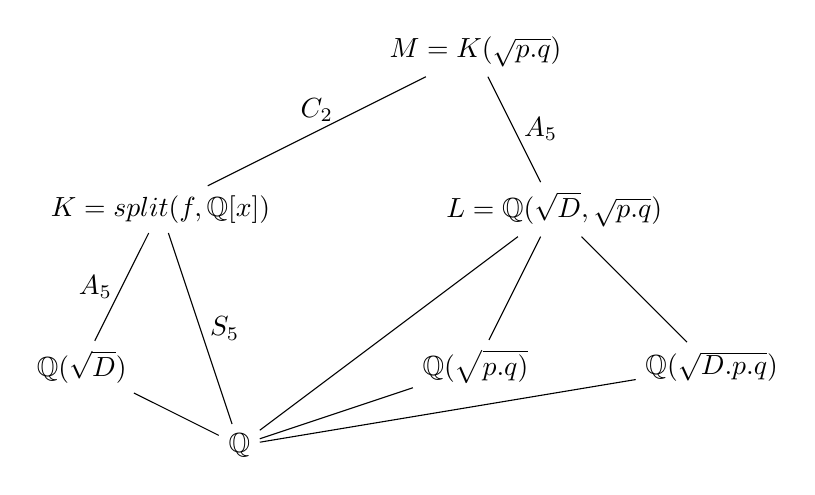
\begin{tikzpicture} [align=center]
  \path  (0, 0)   node(Q)  {$\mathbb{Q}$}
          +(6, 1)   node(QD12) {$\mathbb{Q}(\sqrt{D.p.q})$}
          ++(3,1)   node(Q12) {$\mathbb{Q}(\sqrt{p.q)}$}
           ++(-5,0)   node(QD) {$\mathbb{Q}(\sqrt{D})$}
           ++(1,2)   node(K) {$K=split(f,\mathbb{Q}[x])$}
           ++(5,0)   node(L) {$L=\mathbb{Q}(\sqrt{D},\sqrt{p.q})$}
            ++(-1,2)   node(M) {$M=K(\sqrt{p.q})$};
    \draw [-] (Q) to node [pos=0.5,above]{} (Q12);
    \draw [-] (Q) to node [pos=0.8,below]{} (QD);
    \draw [-] (Q) to node [pos=0.5,below]{} (QD12);
  \draw [-] (QD) to node [pos=0.5,left]{$A_5$} (K);
  \draw [-] (Q) to node [pos=0.5,right]{$S_5$} (K);
  \draw [-] (Q) to node [pos=0.5,below]{} (L);
  \draw [-] (Q12) to node [pos=0.5,below]{} (L);
  \draw [-] (QD12) to node [pos=0.5,below]{} (L);
    \draw [-] (L) to node [pos=0.5,right]{$A_5$} (M);
     \draw [-] (K) to node [pos=0.5,above]{$C_2$} (M);
\end{tikzpicture}
\end{center}

Let r be the number of primes $\mathfrak{p}$ in L ramified in M, and let $\theta$ be a root of f, $T = \mathbb{Q}(\theta)$. \cite{MART1978} shows that M has an infinite 2-class field tower if $r\geq 155$. By assumption p splits completely in T and therefore also in L; furthermore q decomposes in T as $q = \mathfrak{p}_1...\mathfrak{p}_r$, with inertia degrees
\begin{equation}
    (deg(\mathfrak{p}_1),...deg(\mathfrak{p}_r))=\mu 
\end{equation}
Write $Z_\mathfrak{B}\subseteq\Gamma(L/\Q) = S_5$; as the decomposition group of $\mathfrak{B}$ where $\mathfrak{B}$ is a prime in L dividing q. q is unramified so this group is cyclic, and \cite{MART1978} shows that $Z_\mathfrak{B}$ has order at most 3.  It now follows that L has 120 primes dividing p and at least 40 primes dividing q. Then $r\geq 160$ since they all ramify in M, and the theorem follows.
\end{proof}
There are 9 imaginary quadratic fields with class number 1 and 47 imaginary biquadratic number fields with class number 1. Odlyzko's bound (even not assuming GRH) show that no imaginary quadratic number field with trivial class group has an infinite unramified extension. Such a method does not work for imaginary biquadratic number fields with trivial class group, by considering the field $K=\mathbb{Q}(\sqrt{-67},\sqrt{-163})$ which has root discriminant approximately 104.5.

Using SageMath, the following polynomial and primes were found:
\begin{equation}
    f(x)=x^5+4x^4-6x^2-x+1, p=1531,q=71,151,227,\Delta(f)=170701
\end{equation}
\begin{equation}
 f(x)=x^5-4x^4+12x^2-8x+1,p=1987,q=31,107,211,239,\Delta(f)=186037
 \end{equation}
These polynomials satisfy the criteria of the above theorem and therefore describe fields with infinite unramified extensions. Furthermore, the class number of the splitting fields of each of these polynomials is 1, meaning that they are equal to their own Hilbert class fields. \par

\begin{example}
    Using the notation as defined above, \begin{equation}
    f(x)=x^5 - 2x^4 - 20x^3 + 6x^2 + 89x + 67
    \end{equation}
    \begin{equation}
        p=2003,q=499, \Delta(f)=4906992917
    \end{equation}
    Using Magma, the class group of K is isomorphic to $V_4$. Due to the Fundamental Theorem of Galois Theory, there must exist an intermediate field isomorphic to $C_2$ between K and its Hilbert class field. Furthermore, the Hilbert class field of K is isomorphic to the splitting field of \par
   \begin{polynomial}
   x^{20} - 2874x^{18} + 2391847x^{16} -
    471345876x^{14} + 29106648697x^{12} - 550807754260x^{10} +
    4307861945767x^{8} - 14829016524058x^{6} + 23545104859585x^{4} -
    16530672769260x^{2} + 4009653817744
   \end{polynomial}
\end{example}
\begin{example}
    Using the notation as defined above, \begin{equation}
    f(x)=x^5-2x^2-20x^3+6x^2+89x+67
    \end{equation}
    \begin{equation}
        p=811,q=59, \Delta(f)=8996154317
    \end{equation}
    Using Magma, the class group of K is isomorphic to $C_2$. There is no intermediate field isomorphic to  between K and its Hilbert class field. Furthermore, the Hilbert class field of K is isomorphic to the splitting field of \par
   \begin{polynomial}
 x^{10} - 375x^{8} + 5121x^{6} -
    4084x^{4} + 928x^{2} - 64.
   \end{polynomial}
  The splitting field of this polynomial has class group isomorphic to $V_4$.
\end{example}
\subsection{Important Results from Class Field Theory}
\cite{uchida1970} gives the following theorem relating to trinomials:
\begin{theorem}
Suppose $K$ is a number field of finite degree with integers $a$ and $b$, $f(x) = x^n-ax+b$ and $L$ is the splitting field of $f(x)$ over $K$. If $(n-1)a$ and $nb$ are relatively prime, the ramification index of any prime ideal of $L$ over $K$ is either 1 or 2. 
\end{theorem}

This theorem has the following easy corollary:
\begin{corollary}
Suppose $f(x) \in \Q[x]$, with discriminant $D$, and every prime factor in the factorisation of D appears odd times, and let $K$ be the splitting field of $f(x)$ over $\Q$. Then $K/\Q\left(\sqrt{D}\right)$ is unramified.
\end{corollary}
\begin{proof}
Suppose $p$ is a rational prime ramified in $K/\Q$. Then $p|D$. However, $p$ ramifies in $\Q(\sqrt{D})/\Q$, with ramification index 2. Therefore $p$ is unramified in $K/\Q(\sqrt{D})$. 
\end{proof}
\cite{uchida1970} also gives the following examples of unramified extensions of quadratic number fields with Galois group isomorphic to $A_n$.
It is useful to give the following lemma:
\begin{lemma}
Suppose $n$ is prime, and G is a transitive permutation group on $n$ letters , containing a transposition. Then $G$ is a symmetric group.
\end{lemma}

\begin{example}
Define $f_n(x) = x^n-x+1$ with discriminant $D_n$.First note that for all $n \in \mathbb{Z}$. Results from Galois theory show that in the general case, $disc(x^n-ax+n) = n^nb^{n-1}-(n-1)^{n-1}a^n$, and so $D_n = n^n-(n-1)^{n-1}$. For $n$ = 5,6,7, $D_n$ is either prime or the product of two primes, hence $f_n(x)$ satisfies the criteria of the above theorem.  Now 
\begin{equation}
x^5 - x+1 = (x^2 - x +1)(x^3 +x^2 +1) (mod 2)
\end{equation}
hence the Galois group defined by this $f_5(x)$ is symmetric. Similarly arguments hold for n=6 and n=7. Therefore there exist unramified extensions of quadratic number fields with $D_5$, $D_6$, $D_7$ or $S_5$, $S_6$, $S_7$ as Galois groups. 
\end{example}


Now define $g_n(x) = x^n-x-1$ for $ n \in \mathbb{N}$ with discriminant $D_n'$. \cite{SELMER} shows that for $n>1$, $g_n(x)$ is always irreducible. Furthermore, by the above, $D_n'= (-(n-1))^{n-1} - (-n)^{n}$. 
Using Sagemath, the factorisation of $D_n'$ is calculated for $2 \leq n \leq 30$. Define $G_n$ be the Galois group defined by $g_n(x)$. Using the Magma package available at \url{http://magma.maths.usyd.edu.au/calc/}, the Galois group $S_n$ is calculated and all the data is presented in the following table:
\begin{center}
 \begin{tabular}{||c | c | c | c||} 
 \hline
 n & ((n-1)a,nb) & $G_n$ & Factorisation of $D_n'$ \\ [0.5ex] 
 \hline\hline
2 & 1 & $S_{2}$ & 5 \\
\hline
3 & 1 & $S_{3}$ & 23 \\
\hline
4 & 1 & $S_{4}$ & 283 \\
\hline
5 & 1 & $S_{5}$ & 19*151 \\
\hline
6 & 1 & $S_{6}$ & 67*743 \\
\hline
7 & 1 & $S_{7}$ & 776887 \\
\hline
8 & 1 & $S_{8}$ & 11*1600069 \\
\hline
9 & 1 & $S_{9}$ & 7*11*13*43*79*109 \\
\hline
10 & 1 & $S_{10}$ & 173*60042893 \\
\hline
11 & 1 & $S_{11}$ & 275311670611 \\
\hline
12 & 1 & $S_{12}$ & 1237*7438489991 \\
\hline
13 & 1 & $S_{13}$ & 28201*10423708597 \\
\hline
14 & 1 & $S_{14}$ & 31*59*1279*4879633159 \\
\hline
15 & 1 & $S_{15}$ & 52489*418511*19428121 \\
\hline
16 & 1 & $S_{16}$ & 227*246027323*338142271 \\
\hline
17 & 1 & $S_{17}$ & 808793517812627212561 \\
\hline
18 & 1 & $S_{18}$ & 773*1153064743*45072130459 \\
\hline
19 & 1 & $S_{19}$ & 5*659*588489604729898953429 \\
\hline
20 & 1 & $S_{20}$ & 47*233*443*22022174223585405703 \\
\hline
21 & 1 & $S_{21}$ & 1137694897331*5043293621028391 \\
\hline
22 & 1 & $S_{22}$ & 5*69454092876521107983605569601 \\
\hline
23 & 1 & $S_{23}$ & 29*53264767*13296646221023838475181 \\
\hline
24 & 1 & $S_{24}$ & 101*2347*5714547093403974893094772369 \\
\hline
25 & 1 & $S_{25}$ & 10667*282401201*925997749*31362479733103 \\
\hline
26 & 1 & $S_{26}$ & 73*181*2385857*32375941061*6118709648547401 \\
\hline
27 & 1 & $S_{27}$ & 23*3539*535391*10033918834509020645502251401 \\
\hline
28 & 1 & $S_{28}$ & 349*14769635993383*6516302002526983353692617 \\
\hline
29 & 1 & $S_{29}$ & 41393681953973*61230132484136034758796880121 \\
\hline
30 & 1 & $S_{30}$ & 4421*22659339443160463*2080906233684319160584903 \\
\hline


\end{tabular}
\end{center}

Hence for $2 \leq n \leq 30$, the criteria given in the above theorem are fulfilled, and there exist unramified extensions of quadratic number fields with Galois groups isomorphic to $A_n$ or $S_n$ for all such n.  \par


\cite{YAMA1970} gives the following classification of trinomials of the form 
\begin{equation}
    f(x) = x^n+ax+b \in \mathbb{Z}[x]
\end{equation}and K is the splitting field of f over $\Q$.
If the following conditions hold:
\begin{enumerate}
    \item $(n-1).a$ and $n.b$ are relatively prime 
    \item $\Gamma(K/\mathbb{Q}) \cong S_n$
\end{enumerate}\par
Then K is an $A_n$-extension of $\Q\left( \sqrt{\Delta(f)}\right)$ which is unramified at all finite primes.
\begin{lemma}
Suppose $f(x)$ is of the form above, a degree $n$ trinomial If there exist primes $p_1,p_2,p_3$ such that \begin{itemize}
\item $f(x)$ is irreducible modulo $p_1$
\item $f(x)$ is the product of a degree 1 irreducible polynomial and a degree $n-1$ irreducible polynomial module $p_2$
\item $f(x)$ is the product of $n-2$ distinct degree 1 polynomials and a degree 2 irreducible polynomials modulo $p_3$
\end{itemize}
Then the Galois group defined by the splitting field of $f$ is isomorphic to $S_n$.
\end{lemma}
\begin{example}
Set $f(x)= x^5+51x-95$ with discriminant $D$, then $f(x)$ is irreducible modulo 1979, i.e. $f(x)= x^5+51x-95 $ mod 1979, 
$f(x)=(x + 357)(x^4 + 1642x^3 + 1512 x^2 + 1945x + 1338)$ mod 1999, $f(x)=(
x + 194)(x + 384)(x + 1332)(x^2 + 1832x + 950)$ mod 1871. Let $L$ be the splitting field of $f$, and $K = \Q(\sqrt{D(f)})$.    
Note that ((n-1)(a),nb) = (204,-475)=1 and $D = 342859667381 = 7^3 \cdot 11 \cdot 1567 \cdot 57991$. Therefore $\Gamma(L,\Q) \cong S_5$ and $L$ is an $A_5$-extension of $K$ unramified at all finite primes.
\end{example}

% ([1979, 1999, 1871], [-95, 51, 0, 0, 0, 1])
% sage: load("p5.sage")
% ([1999, 1987, 1861], [-58, -23, 0, 0, 0, 0, 1])
% sage: load("p5.sage")
% sage: load("p5.sage")
% ([1999, 1901, 1607], [-60, 114, 0, 0, 0, 0, 0, 1])

Using SageMath, additional examples for degrees 5 and 6 were found:
\begin{example}
Set $f(x)= x^6-23x-58$ with $D$, $K$ and $L$ as above, and $p_1,p_2,p_3$ are equal to 1999,1987,1861 respectively. ((n-1)a,nb) = (-115,-324)=1, $f(x)$ is irreducible mod 1999, $f(x)=(x + 1818)(x^5 + 169x^4 + 743x^3+386x^2+1650x+647)$ mod 1987, $f(x)=(x + 37)(x + 406)(x + 1265)(x+1396)(x^2 + 618 + 1485)$ mod 1861. Also $D = 31085593520933 = 7 \cdot 617 \cdot 7197405307$. Therefore, $\Gamma(L,\Q) \cong S_6$ and $L$ is an $A_6$-extension of $K$ unramified at all finite primes.
\end{example}
In \cite{uchida1970}, further examples are given; for example $x^7-x+1$, $x^9-x+1$ and $x^{10}-x+1$. 
Applying the initial theorem in the case that $n=3$, \cite{uchida1970} also proves that there exist infinitely many real quadratic number fields with class numbers divisible by 3. 

\section{Yamamura's Results}
%todo check this 
\cite{} defines the structure of $\Gamma(K_{ur}/K)$ where K is an imaginary quadratic number field with small conductors. Note that for all number fields with conductor $<1000$, $K_{ur}$ is one of $K_1$, $K_2$ and $K_3$. \par 
Let $K=\Q(\sqrt{d})$ for some integer d. Using Odlyzko's bound as above, the degree $[K^{ur}:K]$ is finite for $|d|\leq 499$, and assuming GRH, replace 499 with 2003. We know that if $[K^{ur}:K_H]<60$, then $K^{ur}=K_H$. However this is difficult to prove; for example for d=-423, $K_H=K_1$. It is necessary to find the degree $[K_H:\Q]$. One way is to use the tower law from Galois theory. Suppose $\Delta(K)=d_1d_2...d_n$, where $\Delta(K)$ is the discriminant of K, then the genus field of K satisfies $K_g=\Q(\sqrt{d_1},\sqrt{d_2},...\sqrt{d_n})$. We have the list of inclusions \begin{equation}
    \Q \subseteq K \subseteq K_g \subseteq K_1 \subseteq (K_g)_1 \subseteq K_2
\end{equation} and the tower law gives \begin{equation}
    [K_2:q] = [K_2:(K_g)_1]h(K_g)[(K_g)_1:\Q]
\end{equation}\par
Here is an explicit example. Let  $d=-1*5*51=-255\equiv \: 1\:mod\:4$. Therefore $|\Delta(K)|=|d|=255$, and $K_g = \Q(\sqrt{5},\sqrt{51}$. Computer verification gives that $h(K_g)=2$, and so \begin{equation}
     [K_2:\Q] = [K_2:(K_g)_1]h(K_g)[(K_g)_1:\Q]= 3*2*4=24
\end{equation}
For d=-255, $K_H=K_2$. We have $cl(K)\equiv C_6 \times C_2$, 

$K_1 = K \left( 
\sqrt{5}, \sqrt[3]{(9+\sqrt{85})/2}
\right)$, $K_2 = K_1 \left( 
\sqrt{2+\sqrt{5}(5+2\sqrt{-3})}
\right)$

 Here $\murgg \cong Q_8 \times C_3$.
\par
$\mathbb{Q}(\sqrt{-1507})$ is the first imaginary quadratic field with an unramified $A_5$-extension over $\mathbb{Q}$. In fact, defining $L=split\left( x^5-5x^3+5x^2+24x+5,\Q\right)$ gives such an $A_5$ extension of K. 
\begin{lemma}
Define $K=\mathbb{Q}(\sqrt{-14731})$, $L=split(x^6+3x^5,5x^4+4x^3+3x^2+2x+1,\mathbb{Q}[x])$. Then L is an unramified $A_6$-extension of K and is an $S_6$ extension of $\mathbb{Q}$.
\end{lemma}
\begin{lemma}
Define $K=\mathbb{Q}(\sqrt{-30759})$, $L=split(x^7+2x^6-3x^4-x^3-x^2-x+2,\mathbb{Q}[x])$. Then L is an unramified PSL(2,7)-extension of K and is an $PSL(2,7)\times C_2$ extension of $\mathbb{Q}$.
\end{lemma}
\subsection{Unramified Galois Extensions of Real Quadratic Number Fields}
%todo check this, write conditions explicitly
In \cite{YAMAMURA2}, we have the following theorem:
\begin{theorem}
    Suppose $S_1$ and $S_2$ are finite sets of primes satisfying $S_1 \cap S_2 = \emptyset$ and $2,5 \notin S_2$. Then there exist infinitely many real quadratic number fields with the following properties: \begin{enumerate}
        \item F is a strictly unramified $A_5$ extension.
        \item All primes in $S_1$ are ramified in F.
        \item All primes in $S_2$ are ramified in F.
    \end{enumerate}
\end{theorem}
To prove this theorem, Yamamura gives the following five conditions for a quintic polynomial of the form \begin{equation}
    f(x)=x^5-2ax^3+bx+c, a,b,c \in \mathbb{Z}
\end{equation}.
\begin{enumerate}
\item f(x) is irreducible over $\Q$.
\item $b \equiv c \equiv 1 \: mod \: 2  $.
\item All the roots of $f(x)$ are real.
\item Define $D$ to be the discriminant of $f$, and define
$A= 5ac^2(3a^2-5b)+8b^2(a^2-b^2)$
$B = 125ac^2-16b(a^2-b)(6a^2-5b)$.
Then any prime factor of $(A,B,D)$ is also a prime factor of $2ac$. 

\item $(a,b,5) =(a^2b-b^2),c,D)=1$.

\end{enumerate} 

\begin{lemma}
Suppose f is as above and the five conditions hold. Then $\Q(\sqrt{D})$ is a real quadratic number field, and the splitting field $K$ of $f(x) $ is a strictly unramified $A_5$-extension of $\Q(\sqrt{D})$. 
\end{lemma}
\begin{example}
    The following example was found using Sagemath. Take a=6,b=-3,c=-7. 
\end{example}
\cite{YAMAMURA2} defines $f_m(x)= x^5-2m^2x^3+(6m^2-1)x-(m-4)$ for some integer $m$. Indeed imposing some modularity conditions on $m$ gives conditions $(2)$ and $(3)$, thereby proving the theorem. 
\cite{YAMAMURA2} also gives examples of real quadratic number fields with class number one having either a strictly or weakly unramified $A_n$-extension which is an $S_n$-extension of $\Q$ for $n$ equal to 5, 6, and 7. Here strictly unramified means that a field extension not ramified at any finite or infinite prime.
\begin{example}
As can be see by Hunter, the minimum possible discriminant a quintic fields with with one real and two pairs of imaginary conjugate field is 1609. 
Taking $K=\Q(\sqrt{1609})$, $h^{+}(K)=1$ and $K$ has a weakly unramified $A_5$ extension
\end{example}
\begin{example}
Suppose $K=\Q(\sqrt{592661})$, then $K$ has a strictly ramified $A_6$ extension, defined by the splitting field of  $x^6 - x^5 - 5x^4 + 4x^3 + 5x^2 - 2^x - 1$. This polynomial is found by using the database of number fields maintained by Jones and Roberts at \cite{JONE2}
%todo find citation and add to bib
\end{example}

\section{Results on Cubics Field Extensions}
In this section, let $K=\Q(\theta)$ where $\theta$ is the root of a cubic polynomial 
f. If $\Gamma(K/\Q) \cong A_3$, call K a  \textbf{cyclic cubic field}.
\begin{proposition}[Galois Theory]
Then K is a cyclic cubic field iff disc(f) is a square. 
\end{proposition} If K is a totally real cubic number field, the (un)conditional bound for the root discriminat given by Odlyzko and published by Martinet is (46.42)72.55. Wong tabulates the all cyclic cubic fields ramified at one prime with trivial class group. 
\begin{example}
    Let $f=x^3-x^2-2x+1$. Then disc(K)=$7^2$, $rd_{k}=3.66$ and h(K)=1. Then unconditionally, K does not have an unsolvable unramified extension, $\Gamma(K:\mathbb{Q})\cong C_3$
\end{example}
\begin{example}
    $f(x)=x^3 + 10x^2 - 9x - 7$, disc(K)=49033, $rd_{K}=36.60$, then unconditionally, K does not have an unsolvable unramified extension, $\Gamma(K:\mathbb{Q})\cong S_3$.
\end{example}


Wong now gives examples of how to calculate the maximal unramified extension of a cyclic cubic field with nontrivial class number. \begin{example}
    $f=x^3-x^2-54x+169$, disc(K)=$163^2$, $rd_{k}=29.84$. Here we have h(K)=4. Define $g(x)=x^6-3x^5-11x^4+27x^3-3x^2-11x+1$. Then John Jones' website gives $L = split(g,\mathbb{Q})$ with $\Delta(K_1)=163^4$. Firstly $\Gamma(L/\mathbb{Q}) \cong A_4$, and 163 is unramified in $L/K$. Hence indeed $L=K_1$. We know that $\Gamma(L/K)\cong V_4$ which is a normal subgroup of $A_4$. Now h(L)=1 and $rd_K < 54.62$ which is the lower bound for the root discriminant of totally real fields of degree 720, certainly $\Gamma(K^{ur}/K) \cong V_4$ and $\Gamma(K^{ur}/\mathbb{Q}) \cong A_4$. 
\end{example}
\begin{example}
K is the cyclic cubic field defined by $x^3-x^2-104x-371$ with $d_K = 313^2$
and $rd_{K} = 46.10$. Now h(K)=7. Define $g(x) = x^7-x^6-15x^5+20x^4+33x^3-22x^2-32x+8$. We can calculate that $K_1=split(g,\Q)$ with field discriminant $313^4$. Since $h(K_1) = 1$ and $rd_K = 46.10 < 56.47$ and 56.47 is the lower
bound for totally real fields of degree 1260, we have $K^{ur}=K_1$ In this
case, we have $\Gamma(K^{ur}/K) \cong C_7$ and $\Gamma(K^{ur}/\mathbb{Q}) \cong F_{21} $.  
\end{example}
Finally consider the results of Golod and Shafarevich as written above. We wish to find a cyclic cubic field with infinite class field tower and infinite unramified extension. Use the following sharp result from Roquette:
\begin{theorem}
    Suppose K is a normal degree n number field, r is the number of infinite places over K, and e(p) be the nonzero exponent of a prime p in the factorisation of n. Let $t_p$ be the number of primes ramified in K with p dividing their ramification index, and $\delta_p$ is 1 if the p-th roots of unity are in K, and 0 otherwise. Then K has an infinite class tower if \begin{equation}
        t_p\geqslant 2 + e(p)\delta_p + \frac{r-1}{p-1} + 2 \sqrt{r+\delta_p}
    \end{equation}
 If K is a cyclic cubic field,  n=r=p=3, e(p)=1, $\delta_3 = 0$. Therefore K has an infinite class tower if $t_3 \geq 3 + 2\sqrt{3} = 6.46$. 
\end{theorem}
Hence we need K to have 7 ramified primes. Here is such an example:
\begin{example}
    Suppose we want K to have discriminant $(3^4)(373^2)(463^2)(547^2)(607^2)(877^2)(997^2)$. Then define $f(x) = x^3 -451235335661981991x-583367691097731940739787$ for $u=12928236$ gives a cyclic cubic field K with 7 ramified primes. Therefore K has an infinite class field tower and infinite unramified extension. 
\end{example}
\section{Serre's Results for Cubic and Quartic}
\subsection{Cubic Example}
Consider the polynomial \begin{equation}
 f(x)=x^3-x-1, \Delta(f)=-23
\end{equation}
Note f has one real root and two imaginary roots. Let L denote its splitting field. Then $\Gamma(L/\mathbb{Q})\cong S_3$ and it is a degree three extension of the quadratic field $K= \mathbb{Q}(\sqrt{-23})$. Now h(K)=3 so using Odlyzko's bounds proves that L is the maximal unramified abelian extension of K. Here is a diagram:
\begin{center}
    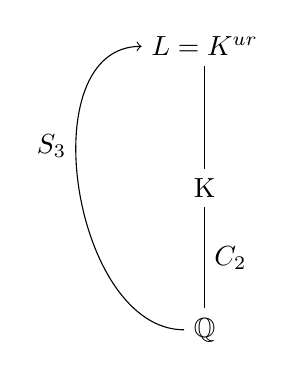
\begin{tikzpicture}[node distance = 1.8cm, auto]
      \node (Q) {$\mathbb{Q}$};
      \node (K) [above of=Q] {K};
      \node (L) [above of=K] {$L=K^{ur}$};
    \draw [->,out=180,in=180,looseness=1] (Q.west) to node[above][pos=0.6,left]{$S_3$}  (L.west);    
    \draw [-] (Q) to node [pos=0.5,right]{$C_2$} (K);
        \draw [-] (K) to node [pos=0.1,left]{} (L);
      \end{tikzpicture}
\end{center}
\subsection{Quartic Example}
Define  \begin{equation}
    f(x)=x^4-x-1, \Delta(f)=-283
\end{equation}
Note f has two real and two imaginary roots. Define L as above and then $\Gamma(L/\mathbb{Q})\cong S_4$. By the fundamental theorem of Galois theory, there exists an intermediate field H corresponding to the normal subgroup $V_4$ of $S_4$. Now $L^H$ is the Hilbert class field of $K= \mathbb{Q}(\sqrt{-283})$ and h(K)=3. Now define a further field extension of L, M such that M is unramified over L (and hence also over K) and M is a Galois extension of $\mathbb{Q}$. Martinet proved that M is the maximal unramified extension of K, with Galois group isomorphic to $SL_2(F_3)$ of order 24. In addition, the Galois group of M over $\mathbb{Q}$ is isomorphic to $GL_2(F_3)$. 
\begin{center}
    \begin{tikzpicture} [align=center]
  \path  (0, 0)   node(Q)  {$\mathbb{Q}$}
          +(4, 1)   node(H) {H}
          +(4,3)   node(L) {L}
          ++(0,6)   node(M) {M}
            +(-4,-3)   node(K) {K};
    \draw [-] (Q) to node [pos=0.5,below]{$A_3$} (H);
    \draw [-] (H) to node [pos=0.5,below]{} (L);
    \draw [-] (Q) to node [pos=0.5,below]{$C_2$} (K);
    \draw [-] (L) to node [pos=0.5,below]{} (M);
    \draw [-] (Q) to node [pos=0.5,below]{$S_4$} (L);
    \draw [-] (Q) to node [pos=0.5,right]{$GL_2(F_3)$} (M);
    \draw [-] (K) to node [pos=0.5,left]{$SL_2(F_3)$} (M);

\end{tikzpicture}
\end{center}


\section{Quintic Extensions}
\subsection{A family of unramified cyclic quintic extensions of imaginary quadratic number fields}
These results are due to \cite{KISH}. For this subsection let $F_n$ denote the n-th Fibonacci number, and $L_n$ the n-th Lucas number. For a non-negative integer m, define $k_m = \Q(\sqrt{-F_{2m+1}})$ and \begin{equation}
    g_m(x) = x^5 - 10x^3  -20x^2 + 
    5(20F^2_{2m+1} - 3)x
    + 40F^2_{2m+1}(-1^{m}L_{2m+1} + 1)- 4
\end{equation} 
Also define \begin{equation}
    \delta_m = 1+\phi^m(\sqrt{-F_{2m+1}})(\zeta-\zeta^{-1})
\end{equation} where $\zeta = e^{\frac{2\pi}{5}}$ and $\phi = \frac{1+\sqrt{5}}{2}$. There exists a unique proper subextension, M, of the bicyclic biquadratic
extension $k(\zeta)/\Q(\sqrt{5})$ which is not equal to $k(\sqrt{5})$ or $\Q(\zeta)$. We denote it by M. Then M is a cyclic quartic field. Define $NT(\alpha) = N_{\Q(\sqrt{5})}(\alpha)Tr_{M/\Q(\sqrt{5})}(\alpha)$. Also define $\tau$ to be the generator of $\Gamma(k(\zeta)/k)$ with $\zeta^2=\zeta^\tau$.
Now for $\gamma \in M$, define the polynomial \begin{equation}
    f_\gamma(x) = x^5 - 10N_M(\gamma)x^3 - 5N_M(\gamma)NT (\gamma)x^2
+ 5N_M(\gamma)(N_M(\gamma) - NT(\gamma^{1+\tau})x - N_M(\gamma)NT(\gamma^{2+\tau}) 
.
\end{equation}
We have the following theorem: \begin{theorem}
    Let m be a non-negative integer and define $E = split(g_m,\Q)$.Then E is a $D_5$-extension
of $\Q$ containing $k_m$. Furthermore, if $m \equiv 12 \:(mod\:52$), then E is an unramified cyclic quintic extension of $k_m$. Therefore, putting $m = 25s + 12$, 5 divides the class number of the quadratic field $\Q(\sqrt{-F_{50s+25}})$.
\end{theorem}
\begin{proof}
Using the result that \begin{equation}
    F_{m+1}= \frac{F_m + L_m}{2}
\end{equation}
we can prove that $f_{\delta_m}(x) = g_m(x)$. Using the fact that $k_m(\zeta)$ is normal over $\Q$, $E\subset k_m(\zeta)$. Now define  \begin{equation}
    \mathcal{M}(k)=\{\gamma \in k(\zeta)^{\times}|\gamma^{3+4\tau+2\tau^{2}+\tau^3}\notin k(\zeta)^5\}
\end{equation}
It therefore holds that $\delta_m \in \mathcal{M}(k_m)$ iff $g_m(x)$ is irreducible over $\Q$. Now both the $\{F_n\}$ and $\{L_n\}$ have periods of length 50 modulo 151. For $m\equiv12 \: mod \: 25$ then \begin{equation}
    g_m(x) \equiv x^5 - 10x^3 - 20x^2 + 65x + 28\:(mod \:151)
\end{equation} which is irreducible over $\Q$. Let $\theta$ be a root of this polynomial. By a result by Sase, no primes are totally ramified over $\Q(\theta)$. Therefore $E/k_m$ is an unramified cyclic quintic extension. 
\end{proof}
\section{Lesseni's Results on Degree 9 Number Fields}
Suppose $K=\mathbb{Q}(\theta)$ is a number field where $\theta$ is a root of an irreducible polynomial of degree 9, and let $L$ represent the Galois closure of K. We have the following theorem: \begin{theorem}
    Suppose GRH holds. Then L cannot be ramified over K only at p=5. Now suppose GRH doesn't hold. Then $5\mathcal{O}_K$ is equal to one of the following: \begin{itemize}
        \item $\mathfrak{p}_1^5\mathfrak{p}_2^4$
        \item $\mathfrak{p}_1^5\mathfrak{p}_2^3\mathfrak{p}_3$
        \item $\mathfrak{p}_1^5\mathfrak{p}_2^2\mathfrak{p}_3^2$
        \item  $\mathfrak{p}_1^5\mathfrak{p}_2^2$
    \end{itemize}
    whence the discriminant $d_K$ is equal to $5^{11}$ or $5^{12}$. 
\end{theorem}
Similar theorems hold for p=3 and p=7.  Using a computer search for primitive number fields defined by a degree 9 polynomial, for a prime $p<11$ there were only 13 distinct number fields found which ramify precisely at 3, and no number fields ramify at 2,5 or 7. However, none of these number fields was primitive, leading to the following conclusion:
\begin{theorem}
    There is no primitive degree 9 number field ramified at only one prime p, $p<11$.
\end{theorem}
\begin{corollary}
 Suppose K is a degree 9 number field which is ramified at only one prime p, $p<11$. Then the Galois group of its Galois closure is solvable. 
\end{corollary}

\section{Kondo's Results}
\begin{theorem}
    Suppose F is a number field with discriminant d(F) of degree n, and K is its Galois closure over $\mathbb{Q}$. Suppose d(F) is not a square, i.e. it is equal to the discriminant of the quadratic number field $\mathbb{Q}(\sqrt{d(F)})$, then \begin{enumerate}
        \item $\Gamma(K:\mathbb{Q})\cong S_n$
        \item $K/\mathbb{Q}(\sqrt{d(F)})$ is an unramified extension.
    \end{enumerate}
\end{theorem}
Furthermore we have the following theorem \begin{theorem}
    The following are equivalent: \begin{enumerate}
        \item d(F) is equal to the discriminant of the quadratic number field $\mathbb{Q}(\sqrt{d(F)})$
        \item For every prime dividing d(F), its ideal $\mathfrak{p}$ in F has precisely one ramified divisor.
    \end{enumerate}
\end{theorem}
\begin{lemma}
Furthermore, the following condition is equivalent to the above:
\par
    The inertia group of every ramified prime of K is a group of order 2 generated by a transposition.\par
In particular, if F satisfies the above condition, then d(F) is equal to $\Delta(\mathbb{Q}(\sqrt{d(F)}))$.
\end{lemma}
\begin{proof}
This is immediate from a theoreom of Van der Waerden. 
\end{proof}
\begin{lemma}
Suppose $d(F)\notin \mathbb{Q}^2$. Then the following are equivalent:\begin{enumerate}
    \item K is an unramified extension of $\mathbb{Q}(\sqrt{d(F)})$
    \item The inertia group of every ramified prime of K is a group of order 2, generated by an odd permutation. 
\end{enumerate}
\end{lemma} 
The following examples were found using SageMath:
\begin{example}
Define $f(x)=x^6 + x^5 - 6x^4 - 4x^3 + 8x^2 + 3x - 2$. Also define $F=\mathbb{Q}(\theta)$, where $\theta$ is a root of f, and let K be the splitting field of f over $\mathbb{Q}$. Then we get $d(f)=\Delta(F)=7846061=17^3.1597$. 
\begin{equation}
   f(x)= (x^3 + 9x^2 + 16x + 7)^2\:modulo\:17
\end{equation}
By the above lemmas, we see that K is an unramified extension of $\mathbb{Q}(\sqrt{17^3.1597})$. Furthermore, $\Gamma(K/\mathbb{Q})$ is a group of order 72 and is isomorphic to the wreath product of $S_3$ and $C_2$. It follows that $K/\mathbb{Q}(\sqrt{17^3.1597})$ is an unramified extension with Galois group isomorphic to the Frobenius group of order 36.
Note the polynomial of degree 6 with the smallest absolute discriminant found was $x^6 - 2x^5 + 2x^4 - x + 1$ with absolute discriminant 11691.
\end{example}
\begin{example}
 Let \begin{equation}
     f(x)=x^7 + 2x^6 - x^5 - x^4 + x^3 - x^2 - x + 1
 \end{equation}and $F$ and $K$ be as above.
Then $d(f)=d(F)=-357911=-71^{3}$ and
\begin{equation}
    f(x)=(x + 19)(x + 42)^2 (x + 59)^2(x + 68)^2\:mod\:71.
\end{equation}
Therefore, by the above Lemma, $K/Q(\sqrt{-71})$ is unramified. The Galois group of $K/Q$
is isomorphic to a dihedral group of order 14, and so $K/Q(\sqrt{-71})$
is an unramified extension with Galois group isomorphic to $C_7$.
This shows that K is the absolute class field of $\mathbb{Q}(\sqrt{-71})$, since $h(Q(\sqrt{-71}))=7$.
\end{example}
\begin{example}
    Suppose we define the polynomial f with the following properties: \begin{equation}
        f(x) =x^9 - x^8 - 2x^7 + x^6 + 2x^5 + x^3 + x^2 - x - 1
    \end{equation} \par
    \begin{equation}
        d(f)=d(F)=66078977=23^3.5431
    \end{equation} 
    \begin{equation}
        f(x)\equiv(x^3 + 8x^2 + 18x + 1)(x^3 + 7x^2 + 3x + 1)^2\:mod\:23.
    \end{equation}
Therefore  $K/Q(\sqrt{-23})$ is unramified. $\Gamma(K/\mathbb{Q})$ is isomorphic to the wreath product of $S_3$ with itself and has order $1296=6^3$, whence $K/Q(\sqrt{-23})$ has Galois group of order 648.
\end{example}

\section{Trying to recreate Maire's Results}
In \cite{MAIR}[3.1] I use Maire's method to find a suitable polynomial.
Firstly, we invoke the following theorem:
\begin{theorem}[Kummer Theory]
Suppose $K/\mathbb{Q}$ is a cyclic extension of degree p,unramified at p, and $L/\mathbb{Q}$ is an extension of degree n. Suppose also that for all places $\mathfrak{Q}$ in L, the ramification index of $\mathfrak{Q}$ in $L/\mathbb{Q}$ divides the ramification index of $\mathfrak{q} = \mathbb{Q}\cap\mathfrak{Q}$ in $K/\mathbb{Q}$. \par
Then the extension $LK/\mathbb{Q}$ is unramified at all finite places. In particular, $\bar{L}K/K$ is also unramified at all finite places.
\end{theorem}
\subsection{Constructing Suitable Polynomials}
Suppose $K$ is a totally real number field of degree $n$ over $\Q$, and $q_1,q_2$ are distinct prime numbers with the following criteria:
\begin{itemize}
\item $Disc(K)$ is equal to some prime $l$.
\item There are precisely $n-2$ unramified places above $l$ in $K/\Q$. 
\item $q_1 \equiv q_2 \equiv \: 3 (4)$.
\item $q_1$ splits completely in $K$.
\item There are precisely $n-1$ unramified places above $q_2$ in $K/\Q$. 
\end{itemize}
Now write $k=\Q(\sqrt{l \cdot q_1 \cdot q_2})$ and $M=Kk$. 
Propositions from \cite{MAIR} give the following inclusions: 
$k = \Q(l \cdot q_1 \cdot q_2) \subset M \subset M_2$.
\subsection{Results}
Using SageMath, the following polynomial and primes were found. Define 
\begin{equation}
    P(x) = x^7-3x^6-5x^5+17x^4+x^3-14x^2+3x+1, l=\Delta(P)=8980833629
\end{equation}
Also define $K=split(P,\mathbb{Q}[x])$. Modulo l,
\begin{eqnarray*}
        P(x)&=&(x+2040911047)(x+3097257563)\\ & & {} (x+3210721157)(x+6041496066)\\ & & {}(x+6737752038)(x+7397598321)^2
\end{eqnarray*}
Now specify values for $q_1$ and $q_2$:
\begin{equation}
    q_1=17471,q_2\in\{443,919,1627,2803,3691,5231,5867,9391\}
\end{equation}
Then indeed $q_1\equiv\:q_2\equiv3(4)$. Also, $q_1$ splits completely in K, and there are n-1 places lying above $q_2$ in $K/\mathbb{Q}$.
\par
Define $L=\mathbb{Q}(\sqrt{l.q_1.q_2})$, $M=KL$. Using the above theorem, all places lying above $q_1$ and $q_2$, in addition to n-2 places above l are ramified in M/K.  Applying \cite{MAIR}[Proposition 2.2] shows that M/L is nowhere ramified. Thus we get the following field extensions
\begin{center}
    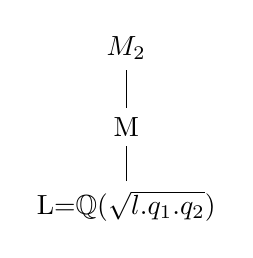
\begin{tikzpicture}[node distance = 1cm, auto]
      \node (L) {L=$\mathbb{Q}(\sqrt{l.q_1.q_2})$};
      \node (M) [above of=L] {M};
      \node (M2) [above of=M] {$M_2$};
      \draw [-] (L) to node {} (M);
      \draw [-] (M) to node {} (M2);
      \end{tikzpicture}
\end{center}
where $M_2/L$ is an infinite unramified extension. We therefore have the following theorem:
\begin{theorem}
    Suppose K is a quadratic field of the form $\mathbb{Q}(\sqrt{8980833629.17471.q_2})$, where 
    \begin{equation}
        q_2\in\{443,919,1627,2803,3691,5231,5867,9391\}
    \end{equation}
    then \begin{enumerate}
        \item $K_H/K$ is finite
        \item $K_\infty/K$ is finite.
    \end{enumerate}
\end{theorem}
\cite{MAIR}[2.1] gives a condition for the p-Hilbert tower of K to be infinite; \cite{MAIR}[2.3] says that if P is an irreducible real polynomial in $\mathbb{Q}[x]$ with squarefree discriminant D(P), and C is its Galois closure, then $C/\mathbb{Q}(\sqrt{\Delta(P)})$ is unramified.
\par
Using these two propositions from Maire can give an algorithm to find a field $K=\mathbb{Q}(\sqrt{l_1.l_2.l_3)}$, where $l_1$ is a prime 1 modulo 4, and $l_2$ and $l_3$ are primes 3 modulo 4. 
\par
Here is an example for n= 5:
\begin{equation}
    x^5 + 12x^4 + 20x^3 - 96x^2 - 4399, D=1255760665676742389.
\end{equation}

\section{Result using Hoelscher}

Using \cite{HOEL} and \cite{JONE}, we see that 
the prime p=239 is tamely ramified for 
\begin{equation}
  G=S_3,G\textsuperscript{ab} = 2, p_w =3  
\end{equation} and also 
\begin{equation}
    G=D_5,G\textsuperscript{ab} = 2 
\end{equation}
This means that we can apply Theorem(1.1) from Hoelscher with
\begin{equation}
    N = G = D_5, K_0 = \mathbb{Q}
\end{equation}
Then 
\begin{equation}
N/p(N) = D_5 \not\subset \mathbb{Z}/(p-1) = \mathbb{Z}_{238}
\end{equation}
We have the field extension diagram
\begin{center}
    
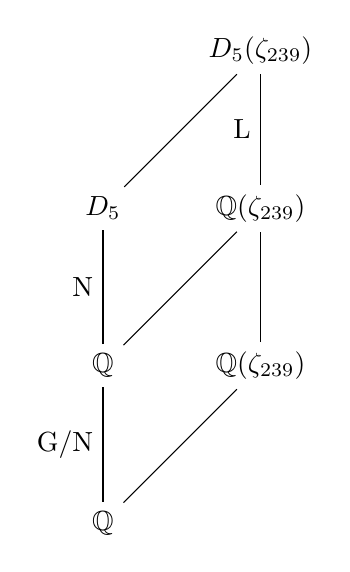
\begin{tikzpicture}[node distance = 2cm, auto]
      \node (Q) {$\mathbb{Q}$};
      \node (K0) [above of=Q] {$\mathbb{Q}$};
       \node (QZP) [above of=Q, right of=Q] {$\mathbb{Q}(\zeta_{239})$};
       \node (K) [above of=K0] {$D_5$};
       \node (K0ZP) [above of=QZP] {$\mathbb{Q}(\zeta_{239})$};
       \node (KZP) [above of=K0ZP] {$D_5(\zeta_{239})$};
       
       \draw[-] (Q) to node {G/N} (K0);
       \draw[-] (K0) to node {N} (K);
       \draw[-] (K) to node {} (KZP);
       \draw[-] (K0ZP) to node {L} (KZP);
       \draw[-] (QZP) to node {} (K0ZP);
       \draw[-] (Q) to node {} (QZP);
       \draw[-] (K0) to node {} (K0ZP);
      \end{tikzpicture}
\end{center}
\par
Where the field extension L is a non-trivial abelian unrafimifed sub-extension of degree prime to p with L Galois over $\mathbb{Q}$.
\subsection{Maire's Results for infinite non Galois unramified extension}
Following from \cite{MAIR}[5.1], there exist infinitely many quadratic fields with a finite 2-Hilbert tower, but having an infinite ramified extension of $2^{\infty{}}$. 
The following methodology was implemented  to find suitable polynomials:
\begin{enumerate}
    \item Pick 8 real numbers close to 0 and define $\tilde{P}(x)$ to be the polynomial with these roots. This is done to increase the probability that P(x) will also have 8 real roots. 
    \item Find a polynomial P(x) which is near to $\tilde{P}(x)$.
    \item Check that the P(x) is irreducible, has 8 real roots and has prime discriminant. 
    \item Search for primes 3 mod 4 which totally decompose in the splitting field of P. 
\end{enumerate}
The following polynomial was found: 
\begin{equation}
    P(X) = (x^8 - 3x^7 - 16x^6 + 31x^5 + 74x^4 - 40x^3 - 56x^2 + 17x + 3)
\end{equation}
where 
\begin{equation}
    l = \Delta(P) = 76363470193820546413
\end{equation}
Put \begin{equation}
    q_1 = 219823, q_2 = 931363, K = split(P, \mathbb{Q}[x]).
\end{equation}
\par
Here $q_1$ and  $q_2$ are totally decomposed in $K/\mathbb{Q}$, the Galois closure of P.
\par
Use the following definitions: 
\begin{itemize}
    \item $N = K\mathbb{Q}(\sqrt{l})$. Note $q_1$ and $q_2$ decompose completely in $N/\mathbb{Q}$, an extension of degree 16.
    \item $E = N(\sqrt{q_1.q_2})$
    \item $E_2$ is the infinite 2-Hilbert tower of E.
\end{itemize}
\par 
We can now draw the following field diagram, where all extensions are unramified 2-extensions. 

\begin{center}
    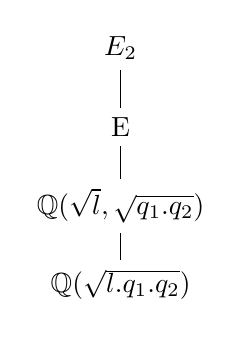
\begin{tikzpicture}[node distance = 1cm, auto]
      \node (Q12) {$\mathbb{Q}(\sqrt{l.q_1.q_2})$};
      \node (QL12) [above of=Q12] {$\mathbb{Q}(\sqrt{l},\sqrt{q_1.q_2})$};
      \node (E) [above of=QL12] {E};
      \node (E2) [above of=E] {$E_2$};
      \draw [-] (Q12) to node {} (QL12);
      \draw [-] (QL12) to node {} (E);
      \draw [-] (E) to node {} (E2);
      \end{tikzpicture}
\end{center}
In fact, $E_2/\mathbb{Q}(\sqrt{l.q_1.q_2})$ is an unramified field extension of degree $2^{\infty}$. Furthermore, the choices of $q_1$ and $q_2$ guarantee that the 2-part of $cl(\mathbb{Q}(\sqrt{q_1.q_2}))$ will be cyclic, and that the 2-Hilbert tower stops at the first extension. 
\begin{theorem}[Cebotarev's Density Criterion]
Let L/K be a finite extension of
number fields with Galois group G, and let $\mathcal{C}$ be a conjugacy class in G. Then the set of
prime ideals of K such that $(\mathfrak{p},L/K)=\mathcal{C}$ has density $|\mathcal{C}|/|G|$ in the set of all prime
ideals of K. If G is abelian, then, for a fixed $\sigma\in G$, the set of prime ideals $\mathfrak{p}$ of K with $\{\mathfrak{p}:(\mathfrak{p},L/K)=\sigma\}$  = (G:1).
\end{theorem}
\begin{corollary}
 If a polynomial $f \in K[x]$ splits into linear factors modulo $\mathfrak{p}$ for all but finitely prime ideals $\mathfrak{p}$ in K, then it splits in $K[x]$.
\end{corollary}
\begin{proof}
Apply the theorem to the splitting field of f.
\end{proof}
Applying this result to the above proves that if the extension K exists, there are infinitely many such $q_1$ and $q_2$ satisfying the conditions.
\section{Kim and Koenig}
\begin{theorem}
 Define $K=\mathbb{Q}(\sqrt{22268})$, $L=split(x^6-10x^4-7x^3+15x^2+14x+3,\mathbb{Q}[x])$. Then $K_1=\mathbb{Q}(\sqrt{76},\sqrt{293})$. Define $M=LK_1$. Then $M=K^{ur}$ and we have the following diagram.   
\end{theorem}
\begin{center}
    \begin{tikzpicture}[node distance = 1.8cm, auto]
      \node (Q) {$\mathbb{Q}$};
      \node (K) [above of=Q] {K};
      \node (K1) [above of=K] {$K_1$};
      \node (M) [above of=K1] {$M=LK_1$};
      \node (L) [right of=K1] {L};
    \draw [->,out=180,in=180,looseness=1] (Q.west) to node[above][pos=0.6,left]{$A_5\times V_4$}  (M.west);    
    \draw [-] (Q) to node [pos=0.1,left]{$C_2$} (K);
    \draw [-] (K) to node {} (K1);
    \draw [-] (K1) to node {$A_5$} (M);
    \draw [-] (Q) to node [pos=0.6,right]{$A_5$} (L);
    \draw [-] (L) to node [pos=0.1,right,above]{$V_4$} (M);
      \end{tikzpicture}
\end{center}
Now define $K=\mathbb{Q}(\sqrt{-1567})$ and 
\begin{equation}
    L=split(x^9-2x^8+10x^7-25x^6+34x^5-40x^4+52x^3-45x^2+20x-4,\mathbb{Q}[x])
\end{equation}Then we use the following theorem
\begin{theorem}
    Write $G=PSL_2(\mathbb{F}_8)$. L is a G-extension of $\mathbb{Q}$; 1567 is the only prime in this field which is ramified with index 2. Abhyankar's Lemma shows that LK/K is unramified at every prime. G is a nonabelian simple group and so $L\cap K_1=\mathbb{Q}$. Therefore $\Gamma(LK_1/K_1)\cong\Gamma(L/\mathbb{Q})\cong G$. It follows that $\Gamma(LK_1/\mathbb{Q})\cong G\times D_{15}$.
\end{theorem}
We have the following diagram:
\begin{center}
    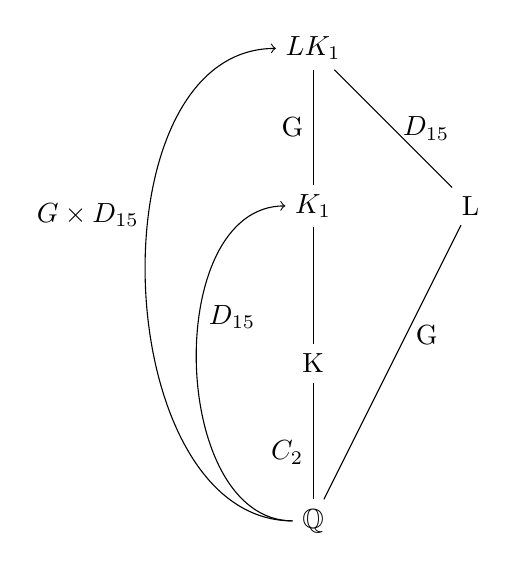
\begin{tikzpicture}[node distance = 2cm, auto]
      \node (Q) {$\mathbb{Q}$};
      \node (K) [above of=Q] {K};
      \node (K1) [above of=K] {$K_1$};
      \node (LK1) [above of=K1] {$LK_1$};
      \node (L) [right of=K1] {L};
    \draw [->,out=180,in=180,looseness=1] (Q.west) to node[above][pos=0.6,left]{$G\times D_{15}$}  (LK1.west);
    \draw [->,out=180,in=180,looseness=1] (Q.west) to node[above][pos=0.6,right]{$D_{15}$}  (K1.west); 
    \draw [-] (Q) to node [pos=0.4,left]{$C_2$} (K);
    \draw [-] (Q) to node [pos=0.6,right]{G} (L);
    \draw [-] (K) to node {} (K1);
    \draw [-] (K1) to node {G} (LK1);
    \draw [-] (L) to node [pos=0.5,right]{$D_{15}$} (LK1);
      \end{tikzpicture}
\end{center}

\section{Using Sympy to find Maximal Unramified Extensions}
Here is an algorithm to find the maximal unramified extension of a number field using Odlyzko's bound and result from Kim \& Koenig and Maire.
\begin{enumerate}
  \item  Order the irreducible quintic polynomial in $\mathbb{Z}[x]$ by the absolute value of their discriminant. 
  \item Pick f(x) to be a possible quintic polynomial.
  \item Calculate $\Delta(f(x))$ and check it is squarefree.
  \item Check that f(x) has precisely three real roots. 
  \item Let S be the splitting field of f, and therefore $\Gamma(S:\mathbb{Q})\cong S_5$
  \item Define $K=\mathbb{Q}(\sqrt{\Delta})$ and therefore $\Gamma(S:K)\cong A_5$. Note by Proposition 2.3 in Maire, S is an unramified extension of K. 
  \item Calculate the root discriminant of K, $rd_K$.
  \item Use the Odlyzko bound to calculate the degree of the maximal unramified extension. If we can show that $[K^{ur}:K]<120$ and $[K^{ur}:\mathbb{Q}]<240$ by the Tower Law, then indeed $K^{ur} = S$.
\end{enumerate}
\par
In fact, we can draw the following diagram: 
\par
\begin{center}
    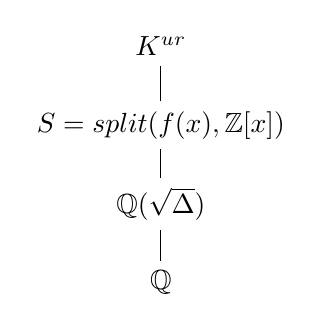
\begin{tikzpicture}[node distance = 1cm, auto]
      \node (Q) {$\mathbb{Q}$};
      \node (K) [above of=Q] {$\mathbb{Q}(\sqrt{\Delta})$};
      \node (S) [above of=K] {$S=split(f(x),\mathbb{Z}[x])$};
      \node (Kur) [above of=S] {$K^{ur}$};
      \draw [-] (K) to node {} (S);
      \draw [-] (Q) to node {} (K);
      \draw [-] (S) to node {} (Kur);
      \end{tikzpicture}
\end{center}
Using Cohn(1955) and verifying with computer search we calculate that a quintic polynomial that satisfies the above conditions, and has minimal absolute discriminant is $f(x) = x^5-2x^3-x^2+1$ which has $\Delta(f) = -4511\equiv1(4)$.
This polynomial has root discriminant = 67.16.
Using the bounds in given in Table(2) of Odlyzko(1990) we find that indeed
\begin{equation}
    \Gamma(K^{ur}:K)\cong A_{5}
\end{equation}
\section{Examples of Maximal Unramified Extension for Quadratic Number Fields}
In this section, GRH is assumed. 
Begin with some definitions:
\begin{definition}
Suppose $G$ is a group. The \textbf{automorphism group} $Aut(G)$ is the group consisting of all the automorphisms of $G$. 

\end{definition}

\begin{definition}
Suppose $N$ and $Q$ are two groups. $G$ is an \textbf{extension} of $Q$ by $N$ if there exists a short exact sequence 
\begin{equation}
1 \rightarrow N \rightarrow G \rightarrow Q \rightarrow 1 
\end{equation}
Such an extension is called a \textbf{central extension} if the centre of $G$ contains $N$. 
\end{definition}
\begin{definition}
A \textbf{p-group} for a given prime number p is a group in which every element has order a power of p.
\end{definition}
The following propoosition from group theory is relevant:
\begin{proposition}
Let $H$ be an abelian 2-group. Suppose that $1 \rightarrow H \rightarrow G \rightarrow A_5 \rightarrow 1$ is a central extension of $A_5$ by $H$. If $|H| > 2$ then $G$ has a non-trivial abelian quotient, whereas if $|H|=2$, then G is isomorphic either to $C_2 \times A_5$ or to $SL_2(F_5)$.
\end{proposition}
The following lemma is a useful result in class field theory:
\begin{lemma}[Abhyankar's Lemma]
    Suppose F is a local field, and $E_1$ and $E_2$ are finite extensions of F with degrees $e_1$ and $e_2$ respectively. In addition, suppose $E_2$ is tamely ramified and $e_2|e_1$. Then $E_1E_2$ is an unramified extension of $E_1$.
 \end{lemma}
 \cite{KIM2017} gives several examples for the determination of the maximal unramified extension of certain quadratic number fields: 
Let $K= \Q(\sqrt{13613})$,  $L$ be the splitting field of $f(x)=x^6-13x^4-7x^3 +44x^2 +40x-9$, and $E$ be a number field defined by a root of $f$, so $L$ is the Galois closure of $E$. Then $f$ has a discriminant of $163^2$ and factorises as
\begin{equation}
(x+4519)(x+6371)^2(x+10315)(x+13438)^2 \: mod \: 13613.
\end{equation}
Therefore $L$ is an $A_5$ extension of $\Q$ unramified only at 13613 with ramification index 2. By Abhyankar's Lemma, $LK/K$ is unramified at all primes. $A_5$ is an nonabelian simple group, so $L \cap K = \Q$ and $\Gamma(LK/K) \cong \Gamma(L/\Q) \cong A_5$, whence $LK$ is an unramified $A_5$-extension of $K$.
Now write $M=LK$. Since $M/K$ is unramified at all places, $M$ and $K$ have the same root discriminant, $rd_M = rd_K = \sqrt{13613} = 116.67 < 121.11 = B(2400,2400,0)$. Therefore $[K^{ur}:M]<20$. \par
Now define $N=KE$, and $N$ is a subfield of $M$, so $N/K$ is unramified. Following the known fact that $N/M \cong D_5$, the Fundamental Theorem of Galois Theory shows that there must exist some intermediate field $F$, $M/F/N$ with $\Gamma(M/F) \cong A_5$ and $\Gamma(F/N) \cong C_2$. Calculation gives that $h(N)=4$ and $cl(N) \cong C_4$, whence $M$ has some unramified $C_2$-extension $T$ with closure $S = \bar{T}$. Therefore $S/M$ is an unramified extension with Galois group $\Gamma(S/M) \cong \left(C_2 \right)^{n}$ for some $1 \leq n \leq 4$. \par
For $n=2$, $|Aut((C_2)^2)| = |C_2| = 2$, and for $n=3$, $|Aut((C_2)^3)| = |PSL(3,2)| = 168$. In either case, the order is not divisible by 60, so $\Gamma(M/K)$ acts trivially on $\Gamma(S/M)$. By the above proposition, $\Gamma(S/K)$ has an abelian quotient, contradicting $h(K)=1$. \par
Now suppose that $m=4$. 
If $\Gamma(M/K)$ acts trivially on $\Gamma(S/M)$, the above proposition will lead to a contradiction. Let $\tilde{N}$ denote the unique intermediate field in $N_2/\tilde{N}/N$, and $\Gamma(N_2/\tilde{N})$ is an abelian quotient of $\Gamma(S/\tilde{N})$. \par 
Noting that  $\Gamma(S/\tilde{N})$ is a $C_5$-extension of
$\Gamma(M/\tilde{N})$ by $\Gamma(S/M) \cong (C_2)^{4})$. Since 
$\Gamma(M/\tilde{N})$ acts nontrivially on $\Gamma(S/M)$
 and it follows that  $\Gamma(S/\tilde{N})$ does not have $C_2$ as a quotient, with contradiction. \par
Therefore, $m = 1$, implying that , $S=T$ and $\Gamma(T/M) = \Gamma(S/M) \cong C_2$. By the above proposition, $\Gamma(T/K) \cong A_5 \times C_2$  or $\cong SL_2(F_5)$ However, $A_5 \times C_2$ has an abelian quotient. Therefore,  $SL_2(F_5)$ is the only possibility. Since Since $T$ is a $\Q$-extension of degree 240, $[K^{ur}:T] < 10$. 

\subsection{p-class Groups of T}

Let $T^p$ be the Hilbert p-class field of T. Since T is Galois over $\Q$, so is $T^p$.
\begin{lemma}
There does not exist a group $G$ with $|G| < 10 $such that $Aut(G)$ contains a subgroup isomorphic to $A_5$ or $SL_2(F_5)$
\end{lemma}
\begin{proof}
Easy check. 
\end{proof}
\begin{corollary}
 $\Gamma(T/K) \cong (SL_2(F_5))$ acts trivially on $\Gamma(T^p/K)$, and so $\Gamma(T^p/K)$ is a central $C_2^N$- extension of $SL_2(F_5)$ by $\Gamma(T^p/T)$. \par
Since $\Gamma(T/M) \cong C_2$, $\Gamma(T^p/M)$ is abelian and $\Gamma(T^p/K)$ is a central extension of $\Gamma(M/K) \cong A_5$ by some abelian group $\Gamma(T^p/M)$.
\end{corollary}
 By the above proposition and corollary, $\Gamma(T^p/K)$ has an abelian quotient, contradicting $h(K)=1$
The above shows, $\Gamma(K^{ur}/T)$ is trivial and so $\Gamma(K^{ur}/K) \cong SL_2(F_5)$. Note that $SL_2(F_5)$ is an unsolvable group. 
 \par
Here are two more examples from \cite{KIM2017}
\begin{example}
Suppose $K = \Q(\sqrt{16621})$ and $f(x) = x^6-13x^4-4x^3 +36x^2 +3x-22$. Then $Disc(f) = 11^2 \cdot 1511^2 = 16621^2$, Define $L= split(f,\Q)$. Then $L$ is an unramified $A_5$-extension of $K$ and similar to the previous example, $\Gamma(K^{ur}/K) \cong SL_2(F_5)$.
\end{example}
\begin{example}
Let K be the real quadratic field Q( 16701). Then, under the assumption of GRH,  $\Gamma(K^{ur}/K) \cong A_5 \times C_2$.
\end{example}
\section{Yamaura Again}
In \cite{YAMA2001}, the table for the $\Q(\sqrt{-d}))^{ur}$ is updated for the missing 19 of the missing 23 values of $d$, apart from $d= -883,-907,-947$. However, if it can be verified that $K^{ur} \neq K_1$ for these fields, then $\Gamma(K^{ur}/K \cong PSL(2,7) \times cl(K)$. 
\cite{YAMA1997} gives the following proposition: \begin{proposition}
For $d=1507 = 11*137$, $\Q(\sqrt{-1507})$ is the first imaginary quadratic number field with an unramified $A_5$-extension which is normal over $\Q$.
Define $f(x) = x^5 -5x^3 + 5x^2 + 24x + 4$, $disc(f) = 581388544 = 2^8 \cdot 11^2 \cdot 137^2$. 
\end{proposition}
Consider now the quadratic number fields defined by $-d = 723, 763, 772, 787,808,843, 904, 932, 939, 964, 971, 979$ with Hilbert class tower of length 1. 
\begin{proposition}
For these fields, if $K$ has odd class number, then $K^{ur} = K_1$. 
\end{proposition}
\begin{proof}
 Conditional Odlyzko bounds give that $[K^{ur}:K_1]<168 = |PSL(2,7)|$, and by results on group extensions from group theory, it is sufficient to show that $K_1$ does not have a unramified $A_5$-extension, normal over $\Q$. Suppose that $K_1$ had such an extension, denoted by $L$. Then $\Gamma(L/K) \cong \Gamma(K_1/K) \times A_5$, and so $K$ would have an unramified $A_5$-extension, normal over $\Q$, contradicting the above proposition. Hence $K^{ur} = K$

\end{proof}
For fields with even class number, for example when $-d = 924 = 2^2 \cdot 241$, existing data for quintic polynomials is used. For $K_1$ to have an unramified $A_5$-extension, normal over $\Q$, it is necessary to find a quintic number field with discriminant $-2^2,241,-2^2 \cdot 241$ or $2^4 \cdot 241$, which does not exist, as can be verified by \cite{JONE2}. Therefore $K^{ue} = K_1$, and the proof for other number fields with even class number are similar. 


\section{Wong}



\bibliographystyle{plain}
\bibliography{my_bibliography.bib}
\end{document}